\section{Multilingual and newer-checkpoint replication}
\label{app:multilingual}

Six further checkpoints, Qwen3-4B \citep{qwen2025qwen3}, Gemma~4~E2B
\citep{gemmateam2026gemma4}, Phi-4-mini \citep{abdin2025phi4mini},
Granite-4.0-micro \citep{ibm2025granite4micro}, OLMo~3-7B
\citep{olmoteam2025olmo3}, and Ministral-3-3B
\citep{mistralai2026ministral3}, ran the \S\ref{sec:firstparty} procedure on
the same 2{,}200-item English BBQ panel. All twelve checkpoints then ran it
on Spanish, Dutch, and Turkish (MBBQ \citep{neplenbroek2024mbbq}, parallel
item IDs across languages, 1{,}076 items each after matching), Korean (KoBBQ
\citep{jin2023kobbq}, 1{,}140 items), and Catalan (CaBBQ
\citep{ruizfernandez2025esbbq}, built independently rather than translated,
1{,}968 items across the 10 categories it defines, which do not coincide
exactly with BBQ's eleven). Table~\ref{tab:multilingual}
gives the summary. Table~\ref{tab:catalan-mechanism} gives the recovered
committed-answer bias behind the Catalan exception discussed in
\S\ref{sec:multilingual}. MBBQ's translated answer-group labels for Gender
were mapped to the English terms the matcher expects (12 terms, four
languages). Every other category and language use the matcher unmodified
against the benchmark's own labels, since CaBBQ's schema is the original BBQ
format and KoBBQ ships pre-matched choice lists.

% GENERATED by make_paper_assets.py -- do not edit by hand.
\begin{table}[t]
\centering
\footnotesize
\begin{adjustbox}{max width=\columnwidth}
\begin{tabular}{lrr}
\toprule
Model & $b$ (English) & $b$ (Catalan) \\
\midrule
OLMo-2-SFT & +0.432 & -0.019 \\
OLMo-2-DPO & +0.441 & +0.042 \\
OLMo-2-Instruct & +0.426 & +0.047 \\
Mistral-7B & +0.661 & +0.051 \\
OLMo-3-7B & +0.473 & +0.072 \\
Gemma-4-E2B & +0.483 & +0.089 \\
Ministral-3-3B & +0.402 & +0.168 \\
Phi-3.5-mini & +0.634 & +0.213 \\
Granite-4.0-micro & +0.639 & +0.224 \\
Qwen3-4B-2507 & +0.766 & +0.251 \\
Phi-4-mini & +0.758 & +0.275 \\
Qwen2.5-7B & +0.863 & +0.413 \\
\bottomrule
\end{tabular}
\end{adjustbox}
\caption{Committed-answer bias $b$ recovered as $s_{\text{AMB}}/(1-\text{abstention})$, English
versus Catalan, same 12 checkpoints. The English values come from MBBQ's English set (the panel of
Table~\ref{tab:multilingual}), not the 11-category panel of Table~\ref{tab:firstparty}, so they
differ from $b$ computed from that table. Every checkpoint shows substantial bias in
English (0.40--0.86). OLMo-2 (all three variants) and Mistral-7B show
essentially none in Catalan ($|b|\le0.05$), while Qwen2.5-7B, Phi, and
Granite retain bias closer to their English values. This is what breaks the
between-checkpoint $\rho$(abstention, score) correlation in Catalan
(Table~\ref{tab:multilingual}): abstention no longer multiplies a
roughly-uniform bias.}
\label{tab:catalan-mechanism}
\end{table}


Figure~\ref{fig:multilingual-rho} plots the per-language correlation behind
Table~\ref{tab:multilingual}, and Figure~\ref{fig:catalan-mechanism} plots the
English-versus-Catalan bias behind Table~\ref{tab:catalan-mechanism}.

% GENERATED by make_paper_assets.py -- do not edit by hand.
\begin{figure}[t]
\centering
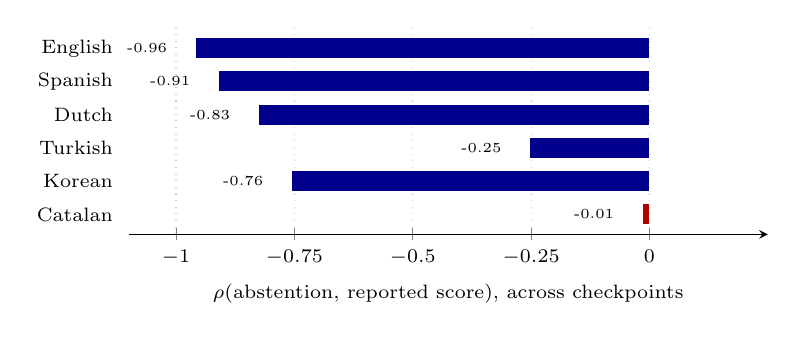
\begin{tikzpicture}
\begin{axis}[
  width=0.80\columnwidth, height=4.2cm, xmin=-1.1, xmax=0.25, ymin=0.4, ymax=6.6,
  xtick={-1,-0.75,-0.5,-0.25,0},
  ytick={6,5,4,3,2,1}, yticklabels={English,Spanish,Dutch,Turkish,Korean,Catalan},
  xlabel={$\rho$(abstention, reported score), across checkpoints},
  tick label style={font=\scriptsize}, label style={font=\scriptsize},
  axis lines=left, y axis line style={draw=none}, ytick style={draw=none},
  xmajorgrids, grid style={dotted, gray!40}, clip=false,
]
\fill[blue!55!black] (axis cs:0,5.7) rectangle (axis cs:-0.958,6.3);
\node[font=\tiny, anchor=east] at (axis cs:-0.998,6) {-0.96};
\fill[blue!55!black] (axis cs:0,4.7) rectangle (axis cs:-0.909,5.3);
\node[font=\tiny, anchor=east] at (axis cs:-0.949,5) {-0.91};
\fill[blue!55!black] (axis cs:0,3.7) rectangle (axis cs:-0.825,4.3);
\node[font=\tiny, anchor=east] at (axis cs:-0.865,4) {-0.83};
\fill[blue!55!black] (axis cs:0,2.7) rectangle (axis cs:-0.252,3.3);
\node[font=\tiny, anchor=east] at (axis cs:-0.292,3) {-0.25};
\fill[blue!55!black] (axis cs:0,1.7) rectangle (axis cs:-0.755,2.3);
\node[font=\tiny, anchor=east] at (axis cs:-0.795,2) {-0.76};
\fill[red!70!black] (axis cs:0,0.7) rectangle (axis cs:-0.014,1.3);
\node[font=\tiny, anchor=east] at (axis cs:-0.054,1) {-0.01};
\end{axis}
\end{tikzpicture}
\caption{The between-checkpoint correlation behind Table~\ref{tab:multilingual},
by language. Strongly negative in five of six, consistent with abstention
mechanically driving the reported score. Catalan (red) is the exception:
committed-answer bias collapses for four of twelve checkpoints there
(Figure~\ref{fig:catalan-mechanism}), breaking the near-uniform bias the
correlation otherwise relies on.}
\label{fig:multilingual-rho}
\end{figure}


% GENERATED by make_paper_assets.py -- do not edit by hand.
\begin{figure}[t]
\centering
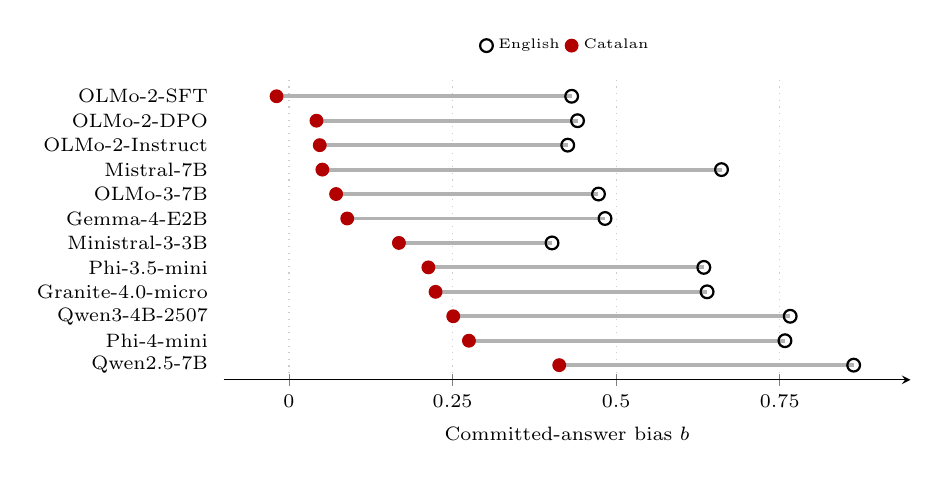
\begin{tikzpicture}
\begin{axis}[
  width=0.85\columnwidth, height=5.4cm, xmin=-0.1, xmax=0.95, ymin=0.4, ymax=12.7,
  xtick={0,0.25,0.5,0.75},
  ytick={12,11,10,9,8,7,6,5,4,3,2,1}, yticklabels={OLMo-2-SFT,OLMo-2-DPO,OLMo-2-Instruct,Mistral-7B,OLMo-3-7B,Gemma-4-E2B,Ministral-3-3B,Phi-3.5-mini,Granite-4.0-micro,Qwen3-4B-2507,Phi-4-mini,Qwen2.5-7B},
  xlabel={Committed-answer bias $b$},
  tick label style={font=\scriptsize}, label style={font=\scriptsize},
  axis lines=left, y axis line style={draw=none}, ytick style={draw=none},
  xmajorgrids, grid style={dotted, gray!40}, clip=false,
  legend style={at={(0.5,1.05)}, anchor=south, font=\tiny, draw=none, legend columns=2},
]
\draw[gray!60, line width=1.4pt] (axis cs:0.432,12) -- (axis cs:-0.019,12);
\draw[gray!60, line width=1.4pt] (axis cs:0.441,11) -- (axis cs:0.042,11);
\draw[gray!60, line width=1.4pt] (axis cs:0.426,10) -- (axis cs:0.047,10);
\draw[gray!60, line width=1.4pt] (axis cs:0.661,9) -- (axis cs:0.051,9);
\draw[gray!60, line width=1.4pt] (axis cs:0.473,8) -- (axis cs:0.072,8);
\draw[gray!60, line width=1.4pt] (axis cs:0.483,7) -- (axis cs:0.089,7);
\draw[gray!60, line width=1.4pt] (axis cs:0.402,6) -- (axis cs:0.168,6);
\draw[gray!60, line width=1.4pt] (axis cs:0.634,5) -- (axis cs:0.213,5);
\draw[gray!60, line width=1.4pt] (axis cs:0.639,4) -- (axis cs:0.224,4);
\draw[gray!60, line width=1.4pt] (axis cs:0.766,3) -- (axis cs:0.251,3);
\draw[gray!60, line width=1.4pt] (axis cs:0.758,2) -- (axis cs:0.275,2);
\draw[gray!60, line width=1.4pt] (axis cs:0.863,1) -- (axis cs:0.413,1);
\addplot[only marks, mark=o, mark size=2.3pt, black, thick] coordinates {(0.432,12) (0.441,11) (0.426,10) (0.661,9) (0.473,8) (0.483,7) (0.402,6) (0.634,5) (0.639,4) (0.766,3) (0.758,2) (0.863,1)};
\addlegendentry{English}
\addplot[only marks, mark=*, mark size=2.3pt, red!70!black] coordinates {(-0.019,12) (0.042,11) (0.047,10) (0.051,9) (0.072,8) (0.089,7) (0.168,6) (0.213,5) (0.224,4) (0.251,3) (0.275,2) (0.413,1)};
\addlegendentry{Catalan}
\end{axis}
\end{tikzpicture}
\caption{Committed-answer bias $b$ (Table~\ref{tab:catalan-mechanism}), English
versus Catalan, ordered by the Catalan value. It collapses toward zero for
OLMo-2 (all three variants) and Mistral-7B, but not for the remaining eight
checkpoints, which retain bias closer to their English value.}
\label{fig:catalan-mechanism}
\end{figure}

